\documentclass[12pt]{article}
%\usepackage[utf8]{inputenc}
%\documentclass[UTF8]{ctexart}
%\usepackage[UTF8, heading = false, scheme = plain]{ctex}
\usepackage{geometry}
%geometry{a4paper,scale=0.9}
\geometry{a4paper,left=1cm,right=1cm,top=1cm,bottom=2cm}
\usepackage{amsfonts}
\usepackage{color}
\usepackage{url}
%\usepackage{biblatex}
\usepackage{amsmath}
\usepackage{amssymb}
\usepackage{latexsym}
\usepackage[linesnumbered,ruled,lined]{algorithm2e}
\usepackage{pythonhighlight}
\usepackage{listings}
\usepackage{cite}
%\addbibresource{ref.bib}
%\bibliography{ref.bib}
\usepackage{caption}
\usepackage{graphicx, subfig}
\usepackage{float}
%\usepackage[fontset=ubuntu]{ctex}
%\usepackage{fontspec}
\usepackage{xeCJK}
%\usepackage[colorlinks,
%anchorcolor=black,
%citecolor=black]{hyperref}
%\setmainfont{SimSun}
\usepackage[section]{placeins}
\usepackage{enumitem}
\usepackage{framed}
\usepackage[framemethod=TikZ]{mdframed}
\usepackage{indentfirst}
\usepackage{setspace}%使用间距宏包
\linespread{1.5}


\title{梯度相关}
%\author{leolinuxer }
%\date{June 2020}

\begin{document}
%\setlength{\parindent}{0pt}
\maketitle
\tableofcontents

\section{泰勒公式和梯度下降法的关系}
见《1-预备知识》

\section{浅谈梯度消失的问题\cite{Commonly_Loss_Functions}}
见《1-预备知识》中的”MSE均方误差+Sigmoid激活函数“和”交叉熵损失+Sigmoid激活函数“。

可以看出,损失函数包含两个部分:1. 计算方法(均方差、交叉熵等);2. 激活函数。

而之前我们遇到的是均方差损失+sigmoid激活函数造成了输出层神经元学习率缓慢,解决思路是交叉熵损失+Sigmoid激活函数;其实我们破坏任意一个条件都有可能解决这个问题:

1. 均方误差损失→交叉熵损失;

2. Sigmoid函数→不会造成梯度消失的函数,例如ReLU函数,不仅能解决输出层学习率缓慢,还能解决隐藏层学习率缓慢问题。

\subsection{ReLU相对于tanh、sigmoid的好处}
第一,采用sigmoid等函数,算激活函数是(指数运算),计算量大;反向传播求误差梯度时,求导涉及除法,计算量相对大。而采用Relu激活函数,整个过程的计算量节省很多。

第二,对于深层网络,sigmoid函数反向传播时,很容易就会出现梯度消失的情况(在sigmoid接近饱和区时,变换太缓慢,导数趋于0),这种情况会造成信息丢失,梯度消失在网络层数多的时候尤其明显,从而无法完成深层网络的训练。

第三,ReLU会使一部分神经元的输出为0,这样就造成了网络的稀疏性,并且减少了参数的相互依存关系,缓解了过拟合问题的发生。

\section{ASGD 收敛性慢的原因}
泰勒展开是在原点附近展开时,收敛性较好;否则收敛性较差,甚至不收敛(见《数学相关/泰勒公式在不同点展开的收敛性讨论》)

\section{梯度验证\cite{Verify_Gradient}}
为了求解一个优化问题,最重要的操作是计算目标函数的梯度。在一些机器学习的应用中,例如深度神经网络,目标函数的梯度公式非常复杂,需要验证自己写出的实现代码是否正确。

\subsection{问题描述}
假设你需要求解优化问题
$$
\min_{w\in\mathbb{R}^2}L(w)
$$

并且用代码实现了求目标函数值和求目标函数梯度的功能。问如何利用求目标函数值的功能来验证求目标函数梯度的功能是否正确?

\subsection{解答和分析}
根据梯度的定义,目标函数的梯度为:
$$
\nabla L(w) = \big[\frac{\partial L(w)}{\partial w_1}, \cdots, \frac{\partial L(w)}{\partial w_n}\big]^T
$$

其中,对于任意的 $i = 1, 2, \cdots, n$,有
$$
\frac{\partial L(w)}{\partial w_i} = \lim_{h\rightarrow 0}\frac{L(w+he_i) - L(w-he_i)}{2h}
$$

其中,向量$e_i$的长度与$w$的长度相同(二者维度相同),仅在第$i$个位置取值为1,其余位置取值为0。因此,我们可以取 $h$ 为一个较小的数(例如 $10^{-7}$),则有:
$$
\frac{\partial L(w)}{\partial w_i} \approx \frac{L(w+he_i) - L(w-he_i)}{2h}
$$

该近似式的左边为目标函数梯度的第$i$个分量,右边仅和目标函数值有关。

下面我们根据泰勒展开及拉格朗日余项公式,有:
$$
L(w+he_i) = L(w) + L'(w)(he_i) + \frac{1}{2} L''(w)(he_i)^2 + \frac{1}{6}L^{(3)}(w)(p_i)(he_i)^3
$$
$$
L(w-he_i) = L(w) - L'(w)(he_i) + \frac{1}{2} L''(w)(he_i)^2 - \frac{1}{6}L^{(3)}(w)(q_i)(he_i)^3
$$

其中,$p_i \in (0,h), q_i \in (-h,0)$。

两个式子相减,等号两边同时除以$2h$,并且因为有$e_i=1$,可得:

$$
\frac{L(w+he_i) - L(w-he_i)}{2h} = \frac{\partial L(w)}{\partial w_i} + \frac{1}{12}(\tilde L^{(3)}(w)(p_i) + \tilde L^{(3)}(w)(q_i))h^2
$$

当 $h$ 较小时,可以近似认为 $h^2$ 项前面的系数为常数 $M$,则近似误差为:
$$
\big|\frac{L(w+he_i) - L(w-he_i)}{2h} - \frac{\partial L(w)}{\partial w_i}\big| \approx Mh^2
$$

当 $h$ 较小时,$h$ 每减小为原来的 $10^{-1}$,近似误差减小为原来的 $10^{-2}$,也就是近似误差是 $h$ 的高阶无穷小。

实际中,我们随机初始化 $w$,取 $h$ 为较小的数(例如 $10^{-7}$),并对 $t = 1, 2, \cdots, n$,验证:
$$
\big|\frac{L(w+he_i) - L(w-he_i)}{2h} - \frac{\partial L(w)}{\partial w_i}\big| <= h
$$
是否成立。如果对于某个下标 $i$,该不等式不成立,那么有两种情况:该下标对应的 $M$ 过大,或者该梯度分量计算不正确。此时可以固定 $w$,减小 $h$ 为原来的 $10^{-1}$,并再次计算下标$i$对应的近似误差。若该近似误差约减小为原来的 $10^{-2}$,则对应于第一种情况,我们应该采用更小的 $h$ 重新做一次验证;否则对应于第二种情况,应该检查求梯度的代码是否有错误。

\section{梯度下降\cite{Common_Gradient_Descent_Algorithms}}
\subsection{常见的梯度下降算法}
梯度下降算法(Gradient Descent Optimization)是神经网络模型训练最常用的优化算法。对于深度学习模型,基本都是采用梯度下降算法来进行优化训练的。梯度下降算法背后的原理:目标函数 $J(\theta)$ 关于参数 $\theta$ 的梯度将是损失函数(loss function)上升最快的方向。而我们要最小化loss,只需要将参数沿着梯度相反的方向前进一个步长,就可以实现目标函数(loss function)的下降。这个步长$\eta$ 又称为学习速率。参数更新公式如下:
$$
\theta \leftarrow \theta - \eta \cdot \Delta J(\theta)
$$

其中 $\Delta J(\theta)$ 是参数的梯度,根据计算目标函数采用数据量的不同,梯度下降算法又可以分为批量梯度下降算法(Batch Gradient Descent),随机梯度下降算法(Stochastic Gradient Descent)和小批量梯度下降算法(Mini-batch Gradient Descent)。对于批量梯度下降算法,其$\Delta J(\theta)$ 是在整个训练集上计算的,如果数据集比较大,可能会面临内存不足问题,而且其收敛速度一般比较慢。随机梯度下降算法是另外一个极端,$\Delta J(\theta)$  是针对训练集中的一个训练样本计算的,又称为在线学习,即得到了一个样本,就可以执行一次参数更新。所以其收敛速度会快一些,但是有可能出现目标函数值震荡现象,因为高频率的参数更新导致了高方差。小批量梯度下降算法是折中方案,选取训练集中一个小批量样本(一般是2的倍数,如32,64,128等)计算,这样可以保证训练过程更稳定,而且采用批量训练方法也可以利用矩阵计算的优势。这是目前最常用的梯度下降算法。

对于神经网络模型,借助于BP算法可以高效地计算梯度,这非常利于采用梯度下降算法对神经网络进行训练。梯度下降算法中一个重要的参数是学习速率,适当的学习速率很重要:学习速率过小时收敛速度慢,而过大时导致训练震荡,而且可能会发散。理想的梯度下降算法要满足两点:收敛速度要快;而且能全局收敛。为了这个理想,出现了很多经典梯度下降算法的变种,下面将分别介绍它们。

\subsubsection{Exponentially weighted moving averages}
在讲各种改进的梯度下降算法之前,我们先简单介绍一下exponentially weighted moving averages,即指数加权移动平均数,因为后面讲到的很多算法要用到这个概念。其针对的序列数据,比如 $t$ 时刻的观测值为 $x(t)$ ,那么评估 $t$ 时刻的移动平均值为:
$$
v(t) \leftarrow \beta \cdot v(t-1) + (1-\beta)\cdot x(t)
$$

其中 $v(t-1)$ 是上一时刻的移动平均值,其实也可以看成历史积累量,一般 $v(0) = 0$,而$\beta$ 是一个系数,其在0~1之间,可以看到移动平均值是按比例合并历史量与当前观测量。现在我们展开上面的式子:
\begin{align*}
v(0) &= 0 \\
v(1) &= \beta \cdot v(0) + (1-\beta)\cdot x(1) \\
v(2) &= \beta \cdot v(1) + (1-\beta)\cdot x(2) = \beta(1-\beta)\cdot x(1) + (1-\beta)\cdot x(2) \\
v(t) &= \beta\cdot v(t-1) + (1-\beta) cdot x(t) = \sum_{i=1}^t\beta^{t-i}(1-\beta)\cdot x(i)
\end{align*}

展开之后,我们可以直观的看到对于每个 $x$ 值,其权重是不一样的,实际上是指数递减的,从当前往后指数递减,所以距离时刻较近的数据会对当前值影响较大,这样计算的好处是平均数会比较平稳。由于权重指数衰减,所以移动平均数只是计算比较相近时刻数据的加权平均数,一般可认为这个时间范围为 $\frac{1}{1-\beta}$,比如 $\beta = 0.9$,你可以近似认为只是平均了10时刻之内的数据而已,因为再往前权重太小了,基本没影响了。如果你熟悉级数的话,也可以计算出权重和是近似为1的,这是在无穷的情况下,但是在前期计算时,权重之和是会小于1的,为了解决这个问题,指数加权移动平均数会引入偏差修正:
$$
v(t) \leftarrow \frac{v(t)}{1-\beta^t}
$$

其实很好理解,就是前期计算时要放大一下计算结果,而后期不需要,此时 $1-\beta^t$ 的值也接近1了。

\subsubsection{Momentum optimization}
冲量梯度下降算法是Boris Polyak在1964年提出的,其基于这样一个物理事实:将一个小球从山顶滚下,其初始速率很慢,但在加速度作用下速率很快增加,并最终由于阻力的存在达到一个稳定速率。对于冲量梯度下降算法,其更新方程如下:
$$
m \leftarrow \gamma \cdot m + \eta \cdot \Delta J(\theta)
$$
$$
\theta \leftarrow \theta - m
$$

可以看到,参数更新时不仅考虑当前梯度值,而且加上了一个积累项(冲量),但多了一个超参 $\gamma$ ,一般取接近1的值如0.9。相比原始梯度下降算法,冲量梯度下降算法有助于加速收敛。当梯度与冲量方向一致时,冲量项会增加,而相反时,冲量项减少,因此冲量梯度下降算法可以减少训练的震荡过程。

有时候,冲量梯度下降算法也可以按下面方式实现:
$$
m \leftarrow \beta \cdot m + (1-\beta) \cdot \Delta J(\theta)
$$
$$
\theta \leftarrow \theta - m
$$

此时我们就可以清楚地看到,所谓的\textbf{冲量项其实只是梯度的指数加权移动平均值}。这个实现和之前的实现没有本质区别,只是学习速率进行了放缩一下而已。

TensorFlow中提供了冲量梯度下降算法的实现:
\begin{python}
#tf.train.MomentumOptimizer(learning_rate=learning_rate, momentum=0.9)
tf.compat.v1.train.MomentumOptimizer(learning_rate=0.05, momentum=0.9)
\end{python}

\subsubsection{Nesterov Accelerated Gradient (NAG)}
NAG算法是Yurii Nesterov在1983年提出的对冲量梯度下降算法的改进版本,其速度更快。其变化之处在于计算“超前梯度”更新冲量项,具体公式如下:
$$
m \leftarrow \gamma \cdot m + (1-\beta) \cdot \Delta J(\theta - \gamma \cdot m) 
$$
$$
\theta \leftarrow \theta - m
$$

既然参数要沿着 $\gamma \cdot m$ 更新,不妨计算未来位置 $\theta - \gamma \cdot m$ 的梯度,然后合并两项作为最终的更新项,可以看到一定的加速效果。在TensorFlow中,NAG优化器为:
\begin{python}
#tf.train.MomentumOptimizer(learning_rate=learning_rate, momentum=0.9, use_nesterov=True)
tf.compat.v1.train.MomentumOptimizer(learning_rate=0.05, momentum=0.9, use_nesterov=True)
\end{python}

\subsubsection{AdaGrad}
AdaGrad是Duchi在2011年提出的一种学习速率自适应的梯度下降算法。在训练迭代过程,其学习速率是逐渐衰减的,经常更新的参数其学习速率衰减更快,这是一种自适应算法。 其更新过程如下:
$$
s \leftarrow s + \Delta J(\theta) \odot \Delta J(\theta)
$$
$$
\theta \leftarrow \theta - \frac{\eta}{\sqrt{s + \varepsilon}} \odot J(\theta)
$$

其中$s$是梯度平方的积累量,在进行参数更新时,学习速率要除以这个积累量的平方根,其中加上一个很小值 $\varepsilon$ 是为了防止除0的出现。由于 $s$是逐渐增加的,那么学习速率是衰减的。考虑如下图所示的情况,目标函数在两个方向的坡度不一样,如果是原始的梯度下降算法,在接近坡底时收敛速度比较慢。而当采用AdaGrad,这种情况可以被改观。由于比较陡的方向 $s$ 比较大,其学习速率将衰减得更快,这有利于参数沿着更接近坡底的方向移动,从而加速收敛。
\begin{figure}[H]
    \centering
    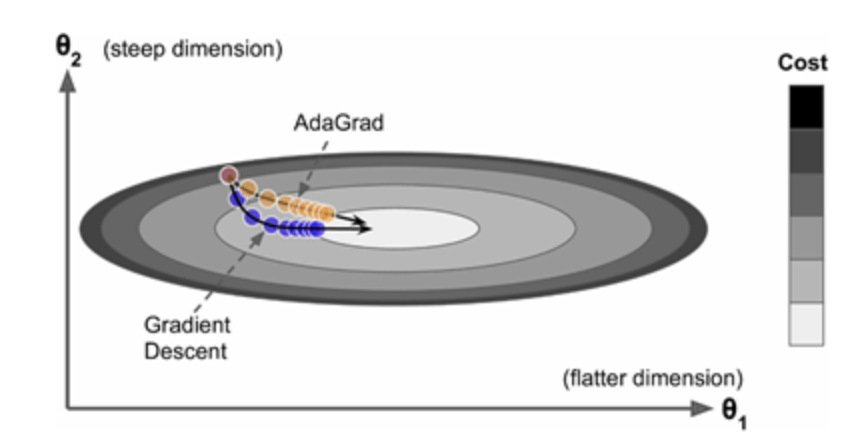
\includegraphics[width=.6\textwidth]{fig/Gradient_Descent_AdaGrad_Example.png}
\end{figure}

AdaGrad其学习速率实际上是不断衰减的,这会导致一个很大的问题,就是训练后期学习速率很小,导致训练过早停止,因此在实际中AdaGrad一般不会被采用,下面的算法将改进这一致命缺陷。
\begin{python}
#tf.train.AdagradOptimizer()
optimizer=tf.optimizers.Adam()
\end{python}

\subsubsection{RMSprop}
RMSprop是Hinton在他的课程上讲到的,其算是对Adagrad算法的改进,主要是解决学习速率过快衰减的问题。其实思路很简单,类似Momentum思想,引入一个超参数,在积累梯度平方项进行衰减:
$$
s \leftarrow \gamma \cdot s + (1-\gamma) \cdot \Delta J(\theta) \odot \Delta J(\theta)
$$
$$
\theta \leftarrow \theta - \frac{\eta}{\sqrt{s + \varepsilon}} \odot J(\theta)
$$

此时可以看到 $s$ 是梯度平方的指数加权移动平均值,其中 $\gamma$ 一般取值0.9,此时 $s$ 更平稳,减少了出现的爆炸情况,因此有助于避免学习速率很快下降的问题。同时Hinton也建议学习速率设置为0.001。RMSprop是属于一种比较好的优化算法了,在TensorFlow中当然有其身影:
\begin{python}
#tf.train.RMSPropOptimizer(learning_rate=learning_rate, momentum=0.9, decay=0.9, epsilon=1e-10)
tf.compat.v1.train.RMSPropOptimizer(learning_rate, decay=0.9, momentum=0.0, epsilon=1e-10, use_locking=False, centered=False, name='RMSProp'
)
\end{python}

\subsubsection{Adadelta}
同时期还有一个Adadelta算法,其也是Adagrad算法的改进,而且改进思路和RMSprop很像,但是其背后是基于一次梯度近似代替二次梯度的思想。

Adadelta解决了Adagrad过度激进地衰减学习率的问题,不同于累加过去所有梯度的平方,它限制了累加的过去的梯度到一个固定窗口宽度 $w$。

为进一步简化存储 $w$ 个梯度的空间消耗,梯度和被递归地定义为之前所有梯度平方的均值的衰减。

详细推导略

\subsubsection{Adaptive moment estimation (Adam)}
Adam是Kingma等在2015年提出的一种新的优化算法,其结合了Momentum和RMSprop算法的思想。相比Momentum算法,其学习速率是自适应的,而相比RMSprop,其增加了冲量项。所以,Adam是两者的结合体:
\begin{align*}
m &\leftarrow \beta_1 \cdot m + (1-\beta_1)\cdot \Delta J(\theta) \\
s &\leftarrow \beta_2 \cdot s + (1-\beta_2) \cdot \Delta J(\theta) \odot \Delta J(\theta) \\
m &\leftarrow \frac{m}{1-\beta_1^t} \\
s &\leftarrow \frac{s}{1-\beta_2^t} \\
\theta &\leftarrow \theta - \frac{\eta}{\sqrt{s+\varepsilon}}\odot m
\end{align*}

可以看到前两项和Momentum和RMSprop是非常一致的, 由于和的初始值一般设置为0,在训练初期其可能较小,第三和第四项主要是为了放大它们。最后一项是参数更新。其中超参数的建议值是: $\beta_1 = 0.9,  \beta_2 = 9.999, \varepsilon = 1e-8$ 。Adm是性能非常好的算法,在TensorFlow其实现如下:
\begin{python}
#tf.train.AdamOptimizer(learning_rate=0.001, beta1=0.9, beta2=0.999, epsilon=1e-08)
tf.compat.v1.train.AdamOptimizer(learning_rate=0.001, beta1=0.9, beta2=0.999, epsilon=1e-08, use_locking=False, name='Adam'
)
\end{python}

\subsection{学习速率}
前面也说过学习速率的问题,对于梯度下降算法,这应该是一个最重要的超参数。如果学习速率设置得非常大,那么训练可能不会收敛,就直接发散了;如果设置的比较小,虽然可以收敛,但是训练时间可能无法接受;如果设置的稍微高一些,训练速度会很快,但是当接近最优点会发生震荡,甚至无法稳定。不同学习速率的选择影响可能非常大。

理想的学习速率是:刚开始设置较大,有很快的收敛速度,然后慢慢衰减,保证稳定到达最优点。所以,前面的很多算法都是学习速率自适应的。除此之外,还可以手动实现这样一个自适应过程,如实现学习速率指数式衰减:
$$
\eta(t) = \eta_0 \cdot 10^{-\frac{t}{r}}
$$

在TensorFlow中,你可以这样实现:
\begin{python}
initial_learning_rate = 0.1
decay_steps = 10000
decay_rate = 1/10
global_step = tf.Variable(0, trainable=False)

learning_rate = tf.compat.v1.train.exponential_decay(initial_learning_rate, 
global_step, decay_steps,
decay_rate)
# decayed_learning_rate = learning_rate *decay_rate ^ (global_step / decay_steps)
optimizer = tf.train.MomentumOptimizer(learning_rate, momentum=0.9)
training_op = optimizer.minimize(loss, global_step=global_step)
\end{python}

\subsection{局部最优和鞍点}
前面说到,我们希望优化算法能够收敛速度快,并且想找到全局最优。对于凸函数来说,其仅有一个极值点,就是全局最优点,此时采用梯度下降算法是可以收敛到最优点的,因为沿着下坡的道路走就可以了。但是其实现在的深度学习模型是一个庞大的非线性结构,这样其一般是非凸函数,存在很多局部最优点(local optimum),一旦梯度下降算法跳进局部陷阱,可以想象其很难走出来,这就很尴尬了,此时梯度下降算法变得不再那么可靠,因为我们想要的是全局最优。很难找到全局最优,这可能是目前优化算法共同面对的问题,如进化算法。不过到底深度学习的损失函数是不是存在很多局部最优点呢?前面所有的分析都是基于低维空间,我们很容易观察到局部最优点。但是深度学习的参数一般庞大,其损失函数已经成为了超高维空间。\textbf{但是Bengio等最新的研究表明,对于高维空间,非凸函数最大的存在不是局部最优点,而是鞍点(saddle point)},鞍点也是梯度为0的点,但是它不像局部最优点或者全局最优点。对于局部最优或者全局最优点,其周围的所有方向要朝向上(最小)或者朝向上(最大),但是考虑到参数庞大,很有可能是一部分方向朝下,一部分方向朝上,这就成为了鞍点。\textbf{意思就是说在高维度空间,不大可能像低维度空间那样出现很多局部最优。而且鞍点也不大可能会成为梯度下降算法的葬身之地}。\textbf{那么真正影响梯度下降算法会是什么呢?可能是平稳区(plateaus),如果出现大面积梯度很小或者近似为0的区域},那么梯度下降算法就找不到方向,想象你自己站在一望无际的平原,估计你也方向感全无了。当前上面所有的谈论仅是停留在经验,对于高维空间,无论如何很难直观想象,这还是一个历史难题吧。

%\printbibliography
\bibliography{../ref}
\bibliographystyle{IEEEtran}
\end{document}